\documentclass{article}
\usepackage{graphicx}
\begin{document}
\section{30P30N static overset scalar verification}
\begin{verbatim}
Problem: three distinct solid profiles (slat, main, flap), normalized chord.
One Gmsh fitted component contains all three physical walls and fluid slots;
a Cartesian background supplies the far field. This is a two-grid case,
not three independently moving fitted grids.

Equation: -Laplacian(u) = -4.
Exact field: u = 1 + x^2 + y^2 + 0.2xy + 0.1x + 0.15y.
Exact Dirichlet data apply only at physical walls and far-field boundaries.
Fringe values are unknowns constrained by ACTIVE donor interpolation.
Nonorthogonal FV fluxes and least-squares gradients are solved together.

Acceptance: both component volume-weighted L2 errors < 3%;
unique physical-domain integrated flux error < 3%; algebraic residual
and actual donor constraints < 1e-10. Independent NumPy replay checks
raw polygons, source profiles, gradients, fluxes and donor constraints.

Scope: scalar equation verification. No overset pressure, velocity, Cp,
lift/drag or turbulence validation is claimed. Point interpolation does
not provide strict local conservative interface flux coupling.

Geometry source: linuxguy123/30P-30N-Validation-Case (GPLv3).
Packaged profile files and exact numerical producer hashes are archived.

Reproduce from the repository:
PYTHONPATH=src python scripts/run_three_element_overset.py --output NEW_DIR
PYTHONPATH=src python scripts/audit_three_element_overset.py NEW_DIR
PYTHONPATH=src python scripts/report_three_element_overset.py NEW_DIR
\end{verbatim}
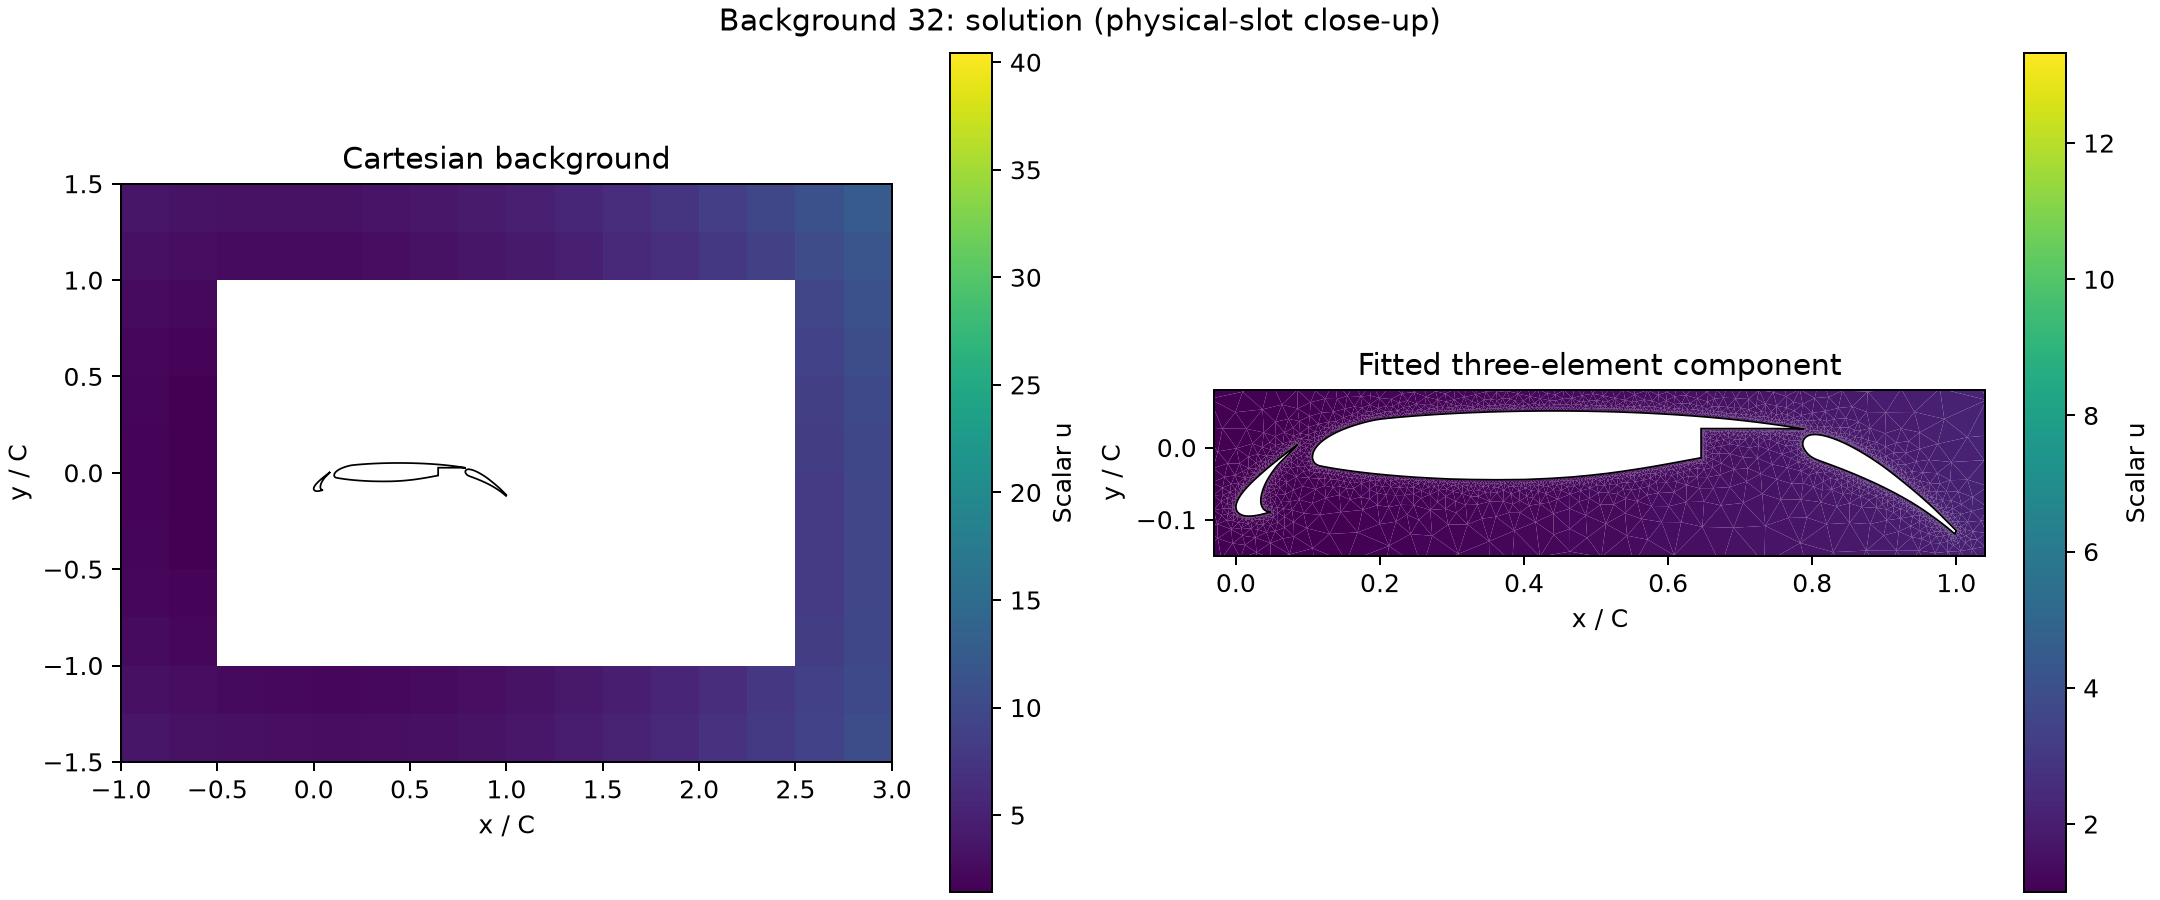
\includegraphics[width=\linewidth]{background-32/solution.png}
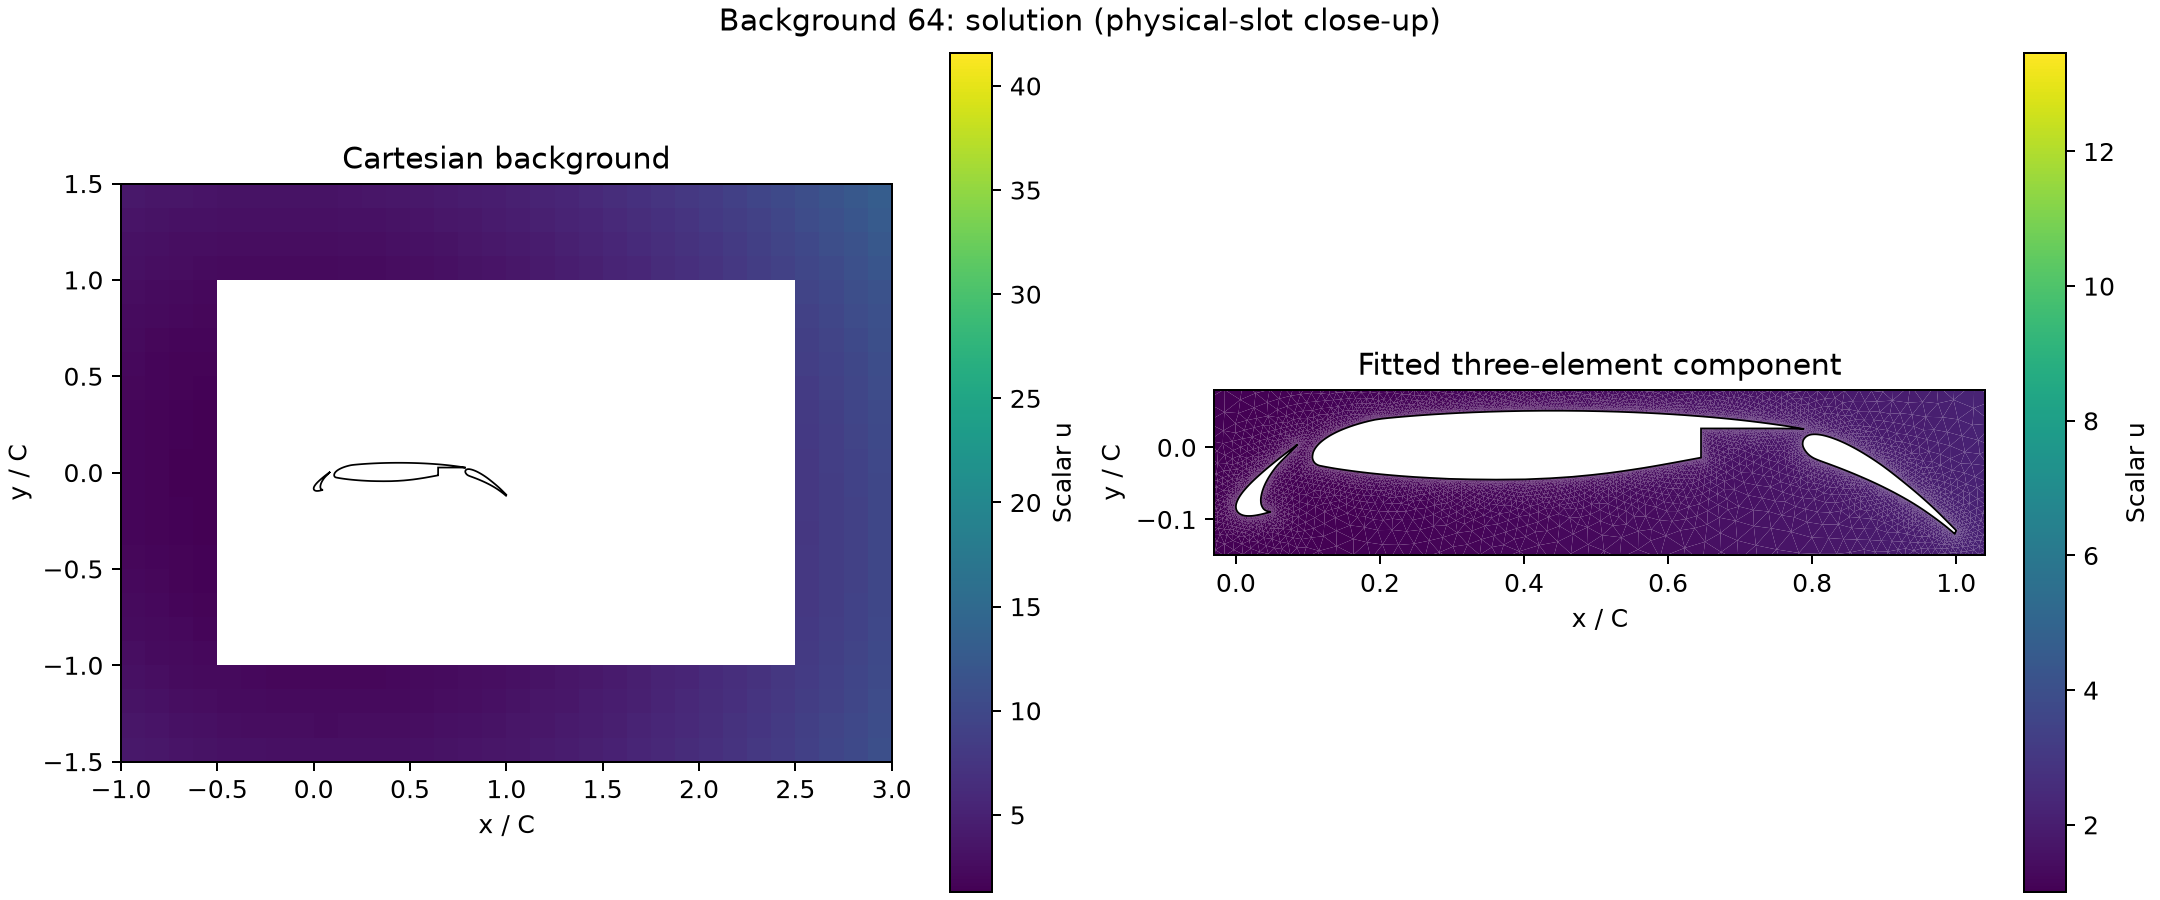
\includegraphics[width=\linewidth]{background-64/solution.png}
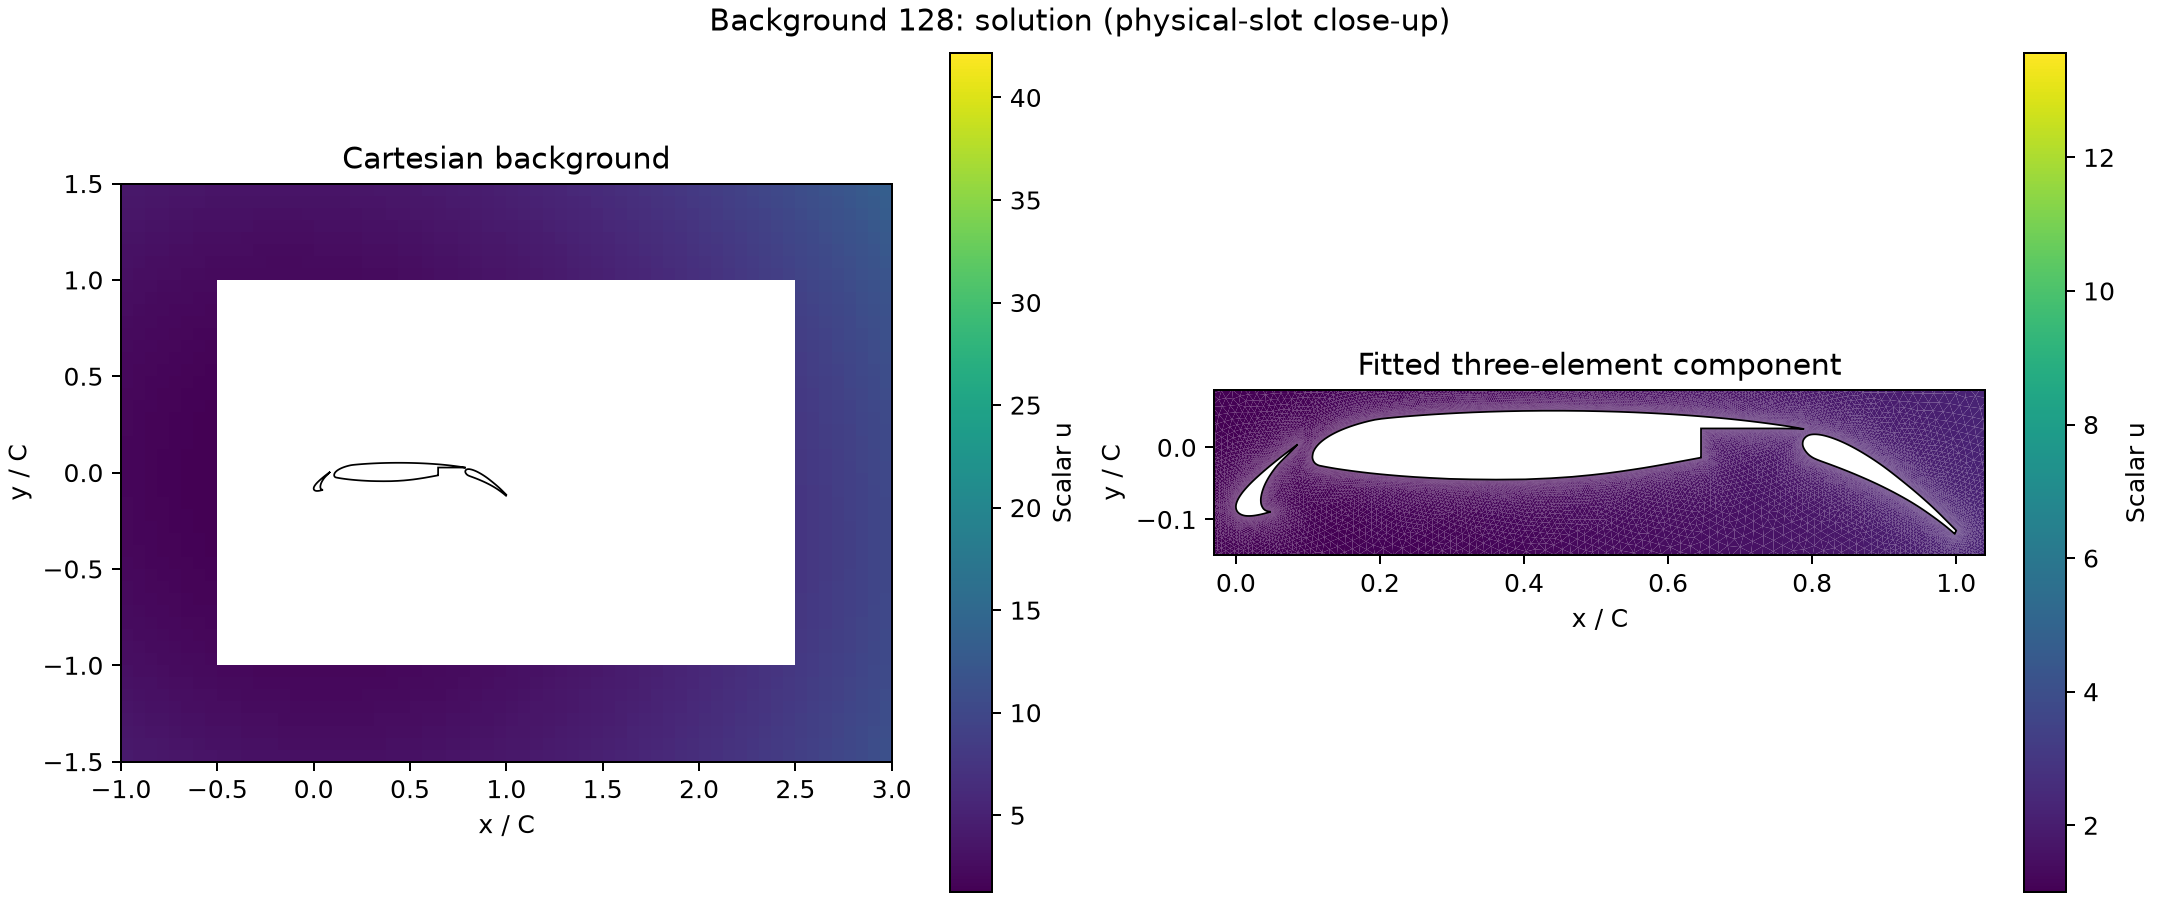
\includegraphics[width=\linewidth]{background-128/solution.png}
\end{document}
